\chapter{Embedded implementation}
\label{ch:Embedded}
In \autoref{ch:Framework}, an overview of the framework developed in \texttt{python} was given, relying on the \gls{glo:mongodb} database. This chapter will focus on the implementation of the embedded system. The first big difference is that the embedded system is written in \texttt{C}, that is not an object oriented language. The second big difference is that the embedded system is not using a database, but it relies only on the variables stored in the RAM. Because of the memory constraints, the training phase relies with the comunication with a \gls{pc} for storing the heavy data. Once the model has been trained, the model is stored in the embedded program and the novelty detection is performed in real time. The general structure is shown in \autoref{fig:Embedded}.

\begin{figure}
    \centering
    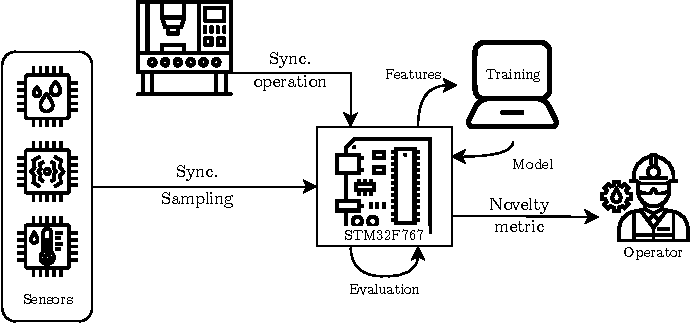
\includegraphics[scale=1]{images/Embedded/EmbeddedStructure.pdf}
    \caption{Embedded system overview}
    \label{fig:Embedded}
\end{figure}


\section{Hardware}
The hardware used for the implementation is the STM32F767ZI board. The characteristics of the board are resumed in \autoref{tab:stm32f767zi}.


\begin{longtable}{p{0.35\linewidth}p{0.55\linewidth}}
    \caption{Hardware characteristics of STM32F767ZI board}    \label{tab:stm32f767zi}\\
    \toprule
    \textbf{Feature} & \textbf{Description} \endfirsthead 
    \hline
    Microcontroller & STM32F767ZI \\
    Architecture & ARM Cortex-M7 \\
    Clock Speed & Up to 216 MHz \\
    Flash Memory & 2 MB \\
    SRAM & 512 KB \\
    EEPROM & No \\
    GPIO & Up to 176 \\
    Timers & 3 x 12-bit, 12 x 16-bit, 2 x 32-bit \\
    ADC & 3 x 12-bit \\
    DAC & 3 x 12-bit \\
    Communication Interfaces & USART, UART, SPI, I2C, CAN, Ethernet, USB \\
    Operating Voltage & 1.7V - 3.6V \\
    Operating Temperature & \SI{-40}{\celsius} to \SI{+150}{\celsius} \\
    \bottomrule    
\end{longtable}

Similarly to what have been done for the \texttt{python} implementation, the parameters of the algorithm are configurable. To avoid the reading of files during the operation, the configuration is held in global variables defined in a header file. The configurable parameters are the usuals: depth of the wavelet three, number of features, sampling frequency, time-series length etc.

\section{Software}
The code consists on a main loop, that is continuously running. It is responsable for executing the state machine behaviour, that manages the different phase of operation. The phases of operation are the same described for the \texttt{python} implementation, except for the training phase, in wich the microcontroller performs the sensor polling, the feature extraction and then send the data to the \gls{pc} using a serial communication. The \gls{pc} is responsable for the training phase. This part is developed again in \texttt{python}, but the final model is then formatted as a \texttt{model.h} file that can be directly included in the embedded code. The model is then stored in the flash memory of the microcontroller, together with the rest of the program.

\subsection{Sensor polling}
\writehereaboutinterrupts

\subsection{Feature extraction}
The features available to be extra are the same as the ones described in \autoref{ch:FeatureExtraction}. The time-domain features are coded directly in a function that is responsible for extracting them. The frequency-domain features are computed by another function that relies on the \texttt{C} library \texttt{wavelib} for the wavelet transform \cite{wavelib}. The power of the wavelet coefficients are then computed and appended to the feature vector. The feature vector is then stored in the RAM, and it is used for the novelty detection.
The features are then standardized using the same mean and standard deviation used for the training phase. The standardization is performed in the same way as in the \texttt{python} implementation.

